% =====================================================================
% Section 4 -- Verification and consistency checks.
% Every number is a macro of paper_numbers.tex; scripts:
%   validation/fig_lumped_validation.py, harrison_case.py, lodewijks_case.py.
% Harrison's mass-spring estimate and the input velocity, the stop of Nordell and
% Ciozda seen from the other side of the take-up, and the comparisons with Lodewijks
% (1996) and Song et al. (2012) in detail are in Appendix C; the wound-rotor drive
% and the stored belt in the supplementary material (S5).
% Lodewijks (1996) adds the mass of the material to the loaded elements: p. 167
% (loaded carry part, element mass = belt plus bulk) and Sect. 8.4.4.
% =====================================================================
\section{Verification and consistency checks}\label{sec:validation}

The solution is checked against a second implementation, against the field records that bear
on its distinctive assumptions, and against a published finite-element model. No record was found
that combines a free gravity take-up, a speed-controlled start, a time history of the take-up and
published conveyor data, so the field checks are partial.

\subsection{Verification against a lumped-mass implementation}\label{sec:lumped}

\begin{figure}[t]
  \centering
  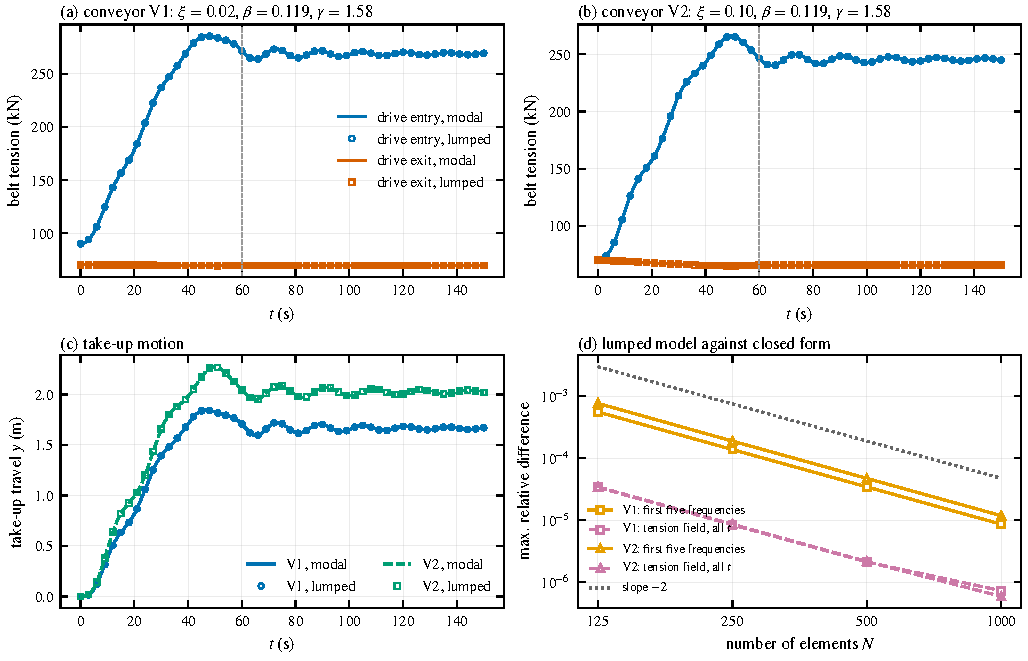
\includegraphics[width=\linewidth]{lumped_validation}
  \caption{Verification against a lumped-mass implementation of the same idealisation.
  (a, b) Total belt tension at the two faces of the drive during a \qty{60}{\second} start to
  \qty{5}{\metre\per\second} of conveyor~V1 (head drive, inclined carry strand, sine profile)
  and conveyor~V2 (drive on the return strand, horizontal, parabolic profile); dashed, end of
  the acceleration. (c) Take-up travel. (d) Largest relative difference between the models
  against the number of elements~$N$, for the first five natural frequencies and for the
  dynamic tension over the loop and time span. Lines: modal solution (120 modes); markers:
  lumped model ($N=\NumLumpedElements$). Illustrative parameters (supplementary material, S4).}
  \label{fig:validation}
\end{figure}

The lumped-mass model (\cref{app:numerics}) shares only the input data with the modal
solution: it uses absolute displacements, so the inertial load of the start emerges instead of
being applied, and starts from a computed static equilibrium. On the two illustrative conveyors
of \cref{fig:validation} the static tensions coincide to round-off. During the
start the dynamic tension over the loop and time span and the take-up travel differ by at most
\num{\NumLumpedTensionErr} and \num{\NumLumpedTravelErr} of their maxima for
$N=\NumLumpedElements$, and the first five natural frequencies by \num{\NumLumpedFreqErr}; the
differences decrease as $N^{-2}$ (observed order \NumLumpedOrder), the discretisation error of
the lumped model. The same agreement holds with the carriage on four strands and with a step
onset of the resistances.
% tests: test_lumped.py (static state, rigid motion, frequencies, starts, step onset),
%        test_strands.py (n = 4 written directly)

\subsection{Consistency with field records}\label{sec:fieldchecks}

\paragraph{Wave speeds} In the stop of a loaded \qty{2.5}{\kilo\metre} conveyor recorded by
\citet{nordell1984}, the two-speed kinematics with their computed wave speeds,
\qty{\NumNCSpeedReturn}{\metre\per\second} empty and \qty{\NumNCSpeedCarry}{\metre\per\second}
loaded, gives arrival times of \qty{\NumNCArrivalB}{\second} and \qty{\NumNCArrivalC}{\second},
against \qty{\NumNCArrivalBMeas}{\second} and \qty{\NumNCArrivalCMeas}{\second} measured. This
reproduces their own comparison and supports (A2), not the take-up model.

\paragraph{The take-up as a free end} \Citet{harrison1983,harrison1985b} recorded the starts
of an empty \qty{5.1}{\kilo\metre} steel-cord conveyor with a \qty{20}{\tonne} gravity take-up
hung on four strands a few tens of metres downstream of the head drive. Two inputs are taken
from the records: the loop transit $L/c_r+L/c_c$, set to the \qty{7}{\second} period of the
elastic waves \citep{harrison1983}, and the wave-speed ratio $\gamma=\NumHarrisonGammaMeas$
measured between three sensors \citep[Fig.~4a]{harrison1985b}; the take-up mass, carried on four strands, then gives
$\beta=\NumHarrisonBetaMin$--$\NumHarrisonBetaMax$ for the two belt densities that his data allow
(\cref{app:validation}). With the take-up
next to the drive, the front returns to the belt beyond it after about one loop transit, so the
arrival time follows from the inputs; the record tests the opacity of the take-up and the slow
period. The carry strand moved
at once, whereas the return belt downstream of the take-up stayed at rest and surged away
\qty{\NumHarrisonStillMeas}{\second} later \citep[Fig.~2b]{harrison1985b}. In the model the
take-up transmits only $|\chi|=\NumHarrisonTransmissionMin$--$\NumHarrisonTransmissionMax$ of a
wave with the period of the elastic waves, and the return belt beyond it stays below
\qty{\NumHarrisonStillSpeed}{\metre\per\second} until the front arrives, after
\qty{\NumHarrisonTransit}{\second}. With a hydraulic buffer under the carriage the two belts
moved away together \citep[Fig.~3b]{harrison1985b}, as Eq.~\eqref{eq:transmission_z} predicts
for a stiff belt-side impedance, although that modification also changed other parts of the
design. A stop recorded by \citet{nordell1984}, whose take-up had a hydraulic retarder, is
consistent with the same opacity (\cref{app:validation}).

\paragraph{The slow take-up period} After the start the take-up oscillated with a period of
\qty{25}{\second} \citep{harrison1983} (\qty{\NumHarrisonSlowMeas}{\second} in our read-out of
his Fig.~5e). The model gives \qty{\NumHarrisonSlowModel}{\second},
\qty{\NumHarrisonSlowExcess}{\percent} longer, the quarter-wave period of strand~B with the
take-up as a free end, almost independent of the take-up mass; an embedded-mass model with the
same loop transit gives at most \qty{\NumHarrisonEmbeddedMax}{\second}. The record is
compatible only with a nearly free end. The remaining difference, and an elastic ripple that the
model lacks, point to the wound-rotor drive, started by torque steps: with Eq.~\eqref{eq:chareq_torque}
a free drive gives the ripple, as the loop transit (\qty{\NumHarrisonFreeDriveSecond}{\second}),
and a reduced drive mass \NumHarrisonDriveMassBeltRatio\ times that of the belt gives the slow
period, but no single linear drive gives both (supplementary material, S5). The record does not
test the value of $\beta$.
% validation/harrison_case.py (summary, drive_check)

\subsection{Cross-comparison with a finite-element model}\label{sec:lodewijks}

Set up from the data of \citet[Ch.~8]{lodewijks1996}, the model reproduces the peak belt
strains of his five speed-controlled starts of a loaded \qty{1}{\kilo\metre} conveyor (30 to
\qty{35}{\second}) within \qty{\NumLodewijksPeakDevMin}{\percent} to
\qty{\NumLodewijksPeakDevMax}{\percent} (\cref{app:validation}), but not the oscillation after
the start: \qty{\NumLodewijksPeriodMeas}{\second} in our fit of his Figs.~8.41--8.42, against
\NumLoPeriodLow--\qty{\NumLodewijksPeriodModel}{\second} over the coupling range of the
material. A period near his would need a carry strand without the inertia of the material
(\qty{\NumLodewijksPeriodEmpty}{\second}), but his model adds the mass of the material to the
loaded elements \citep[\S8.4]{lodewijks1996}, or a drive without speed control
(\qty{\NumLodewijksPeriodOwnDrive}{\second}), but in his starts the drive speed follows the set
point \citep[Fig.~8.38]{lodewijks1996}. His model also merges the drive and the take-up into a
single moving pulley \citep[\S7.2, Eq.~7.55]{lodewijks1996}. If the drive faces moved with the
carriage, the period would be \qty{\NumLodewijksPeriodSliding}{\second}
(\qty{\NumLodewijksPeriodSlidingLow}{\second} at the weakest coupling), but half of the drive force
would then unload the return belt, whose tension at the take-up would swing
between \NumLodewijksSlackSlidingMin\ and \qty{\NumLodewijksSlackSlidingMax}{\kilo\newton} in his
offset start; in his Fig.~8.41 it stays between \NumLodewijksSlackHisMin\ and
\qty{\NumLodewijksSlackHisMax}{\kilo\newton}, as with a take-up that holds the slack side
(\cref{app:validation}). The discrepancy is unresolved. The agreement of the peaks is a
cross-check between models of different scope, not a validation of either;
Section~\ref{sec:application} separates what depends on the fundamental period of this conveyor
from what does not.
% validation/lodewijks_case.py, data/lodewijks_case.json
